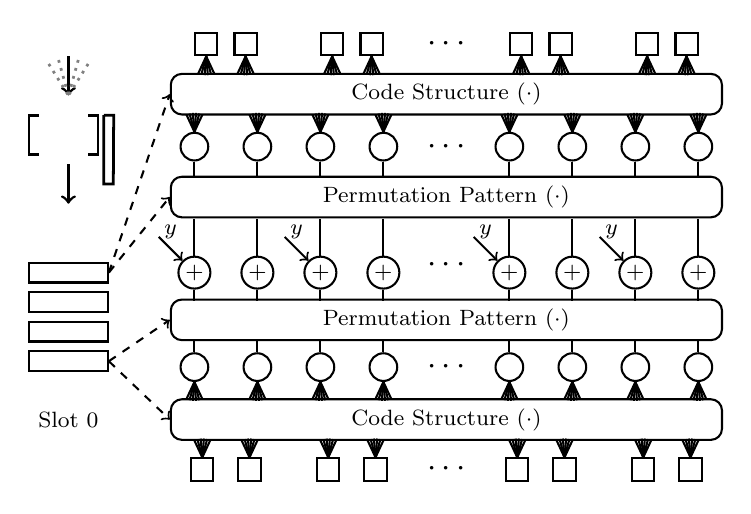
\begin{tikzpicture}
[font=\footnotesize, draw=black, line width=0.75pt,
bitnode/.style={circle,minimum size=10pt,draw=black},
checknode/.style={rectangle,minimum size=8pt,draw=black},
bigPerm/.style={rectangle,draw,minimum width=7cm, minimum height=5mm,rounded corners,draw=black},
sub0/.style={rectangle, draw, inner sep=0pt, minimum width=10mm, minimum height=2.5mm}
]

\def \tcny {2.9}
\def \tvny {1.6}
\def \gmacy {0}
\def \bvny {-1.2}
\def \bcny {-2.5}

\foreach \v in {-2.0} {
  \draw[->, line width=1pt]  (\v,2.75) -- (\v,2.25);
  \draw[dotted, line width=1pt, draw=gray]  (\v-0.25,2.65) -- (\v,2.25);
  \draw[dotted, line width=1pt, draw=gray]  (\v-0.125,2.7) -- (\v,2.25);
  \draw[dotted, line width=1pt, draw=gray]  (\v+0.125,2.7) -- (\v,2.25);
  \draw[dotted, line width=1pt, draw=gray]  (\v+0.25,2.65) -- (\v,2.25);

  \draw[line width=1pt] (\v-0.375,2) -- (\v-0.5,2) -- (\v-0.5,1.5) -- (\v-0.375,1.5);
  \draw[line width=1pt] (\v+0.25,2) -- (\v+0.375,2) -- (\v+0.375,1.5) -- (\v+0.25,1.5);
  \draw[line width=1pt] (\v+0.45,2) -- (\v+0.45,1.125) -- (\v+0.57,1.125) -- (\v+0.575,2) -- (\v+0.45,2);

  \draw[->, line width=1pt]  (\v,1.375) -- (\v,0.875);
}

\foreach \c/\l in {0/1, -0.375/2, -0.75/3, -1.125/4} {
  \node[sub0] (subcs\l) at (-2,\c) {};
}

\foreach \x/\i in {0/1,2/2,5/3,7/4} {
% Top Check Nodes
  \node[checknode] (tbcna\i) at (0.8*\x-0.25, \tcny) {};
  \node[checknode] (tbcnb\i) at (0.8*\x+0.25, \tcny) {};

% Top Variable Nodes
  \node[bitnode] (tvna\i) at (0.8*\x-0.4, \tvny) {};
  \node[bitnode] (tvnb\i) at (0.8*\x+0.4, \tvny) {};

% GMAC Code Symbols
  \node[bitnode,inner sep=1pt] (gmaca\i) at (0.8*\x-0.4, \gmacy) {$+$};
  \node[bitnode,inner sep=1pt] (gmacb\i) at (0.8*\x+0.4, \gmacy) {$+$};

% Bottom Variable Nodes
  \node[bitnode] (bvna\i) at (0.8*\x-0.4, \bvny) {};
  \node[bitnode] (bvnb\i) at (0.8*\x+0.4, \bvny) {};

% Bottom Check Nodes
  \node[checknode] (bcna\i) at (0.8*\x-0.3, \bcny) {};
  \node[checknode] (bcnb\i) at (0.8*\x+0.3, \bcny) {};

% Edges - Set 1
  \foreach \angle in {65,75,85,95,105,115} {
    \draw (tvna\i.north) -- +(\angle:0.24);
    \draw (tvnb\i.north) -- +(\angle:0.24);
    \draw (bcna\i.north) -- +(\angle:0.24);
    \draw (bcnb\i.north) -- +(\angle:0.24);
    }

% Edges - Set 2
  \foreach \angle in {245,255,265,275,285,295} {
    \draw (tbcna\i.south) -- +(\angle:0.24);
    \draw (tbcnb\i.south) -- +(\angle:0.24);
    \draw (bvna\i.south) -- +(\angle:0.24);
    \draw (bvnb\i.south) -- +(\angle:0.24);
    }

  \draw (gmaca\i.south) -- +(0,-0.14);
  \draw (gmacb\i.south) -- +(0,-0.14);
  \draw (gmaca\i.north) -- +(0,0.47);
  \draw (gmacb\i.north) -- +(0,0.46);

  \draw (bvna\i.north) -- +(0,0.15);
  \draw (bvnb\i.north) -- +(0,0.15);
  \draw (tvna\i.south) -- +(0,-0.18);
  \draw (tvnb\i.south) -- +(0,-0.18);

  \draw[<-] (gmaca\i.north west) -- node[midway, above]{$y$} +(-0.3,0.3);
}

  \node at (2.8,\tcny) {\large $\cdots$};
  \node at (2.8,\tvny) {\large $\cdots$};
  \node at (2.8,\gmacy+0.1) {\large $\cdots$};
  \node at (2.8,\bvny) {\large $\cdots$};
  \node at (2.8,\bcny) {\large $\cdots$};

  \node[bigPerm] (tvn2cny) at (2.8,0.4875*\tvny+0.5125*\tcny) {Code Structure $(\cdot)$};
  \node[bigPerm] (tvn2gmacy) at (2.8,0.6*\tvny+0.4*\gmacy) {Permutation Pattern $(\cdot)$};
  \node[bigPerm] (bvn2gmacy) at (2.8,0.5*\gmacy+0.5*\bvny) {Permutation Pattern $(\cdot)$};
  \node[bigPerm] (bvn2cny) at (2.8,0.4875*\bvny+0.5125*\bcny) {Code Structure $(\cdot)$};

  \node (slot0) at (-2,0.4875*\bvny+0.5125*\bcny) {Slot 0};

\draw[->,dashed] (subcs1.east) -- (tvn2cny.west);
\draw[->,dashed] (subcs1.east) -- (tvn2gmacy.west);

\draw[->,dashed] (subcs4.east) -- (bvn2cny.west);
\draw[->,dashed] (subcs4.east) -- (bvn2gmacy.west);
\end{tikzpicture}
